\documentclass[11pt]{article}
% Font & ngôn ngữ tiếng Việt (pdfLaTeX)
\usepackage[utf8]{inputenc}
\usepackage[T5]{fontenc}


% Biblatex + biber
\usepackage[backend=biber, style=numeric-comp, autolang=other]{biblatex}
% GIẢ SỬ BẠN CÓ TỆP NÀY:
\addbibresource{references.bib}

% Toán học & font Times
\usepackage{amsmath, amssymb, amsfonts, bm}

% Bảng biểu & căn lề
\usepackage{longtable}
\usepackage{array}
\usepackage{booktabs}

% Đồ họa & màu sắc
\usepackage{graphicx}
\usepackage{xcolor}
\usepackage{float}
\usepackage{subcaption}

% Liên kết & tham chiếu
\usepackage{hyperref}
\hypersetup{
    colorlinks=true,
    linkcolor=blue,
    urlcolor=red,
    pdftitle={Overleaf Example},
    pdfpagemode=FullScreen,
}

% Dấu tick và x
\usepackage{pifont}
\newcommand{\xmark}{\ding{55}}
\newcommand{\cmark}{\ding{51}}

% Tiêu đề tùy chỉnh
\usepackage{titling}
\setlength{\droptitle}{-10em}
\renewcommand{\maketitle}{%
    \begin{center}
        \fontsize{18}{20}\selectfont\textbf{Quản lý Phiên bản Dữ liệu (DVC) \\[0.2em] trong các Dự án Machine Learning}\\[1em]
        \fontsize{14}{16}\selectfont Nhóm MLOps\\[0.5em]
        \fontsize{14}{16}\selectfont Ngày 18 tháng 10 năm 2025
    </end{center}
    \vspace{1.5em}
}

% Format section (không đánh số)
\usepackage{titlesec}
\titleformat{\section}{\normalfont\Large\bfseries}{}{0em}{}

% Code block
\usepackage{listings}
\definecolor{backcolour}{rgb}{0.95,0.95,0.92}
\lstset{
    backgroundcolor=\color{backcolour},
    basicstyle=\ttfamily\footnotesize,
    breaklines=true,
    numbers=left,
    numberstyle=\tiny\color{gray},
    captionpos=b,
    language=bash, % Đặt ngôn ngữ mặc định là bash cho lstlisting
    morekeywords={python, dvc, git, conda, mkdir, cd, pip, mklink, del}, % Thêm keywords
    commentstyle=\color{gray}, % Màu cho comment
    keywordstyle=\color{blue},
    stringstyle=\color{red}
}

% Hộp màu
\usepackage[many]{tcolorbox}
\definecolor{lightgreenbox}{rgb}{0.85,0.95,0.85}
\newtcolorbox{summarybox}{
    colback=lightgreenbox,
    colframe=green!50!black,
    boxsep=5pt, arc=4pt,
    boxrule=0.5pt,
    left=10pt, right=10pt,
    top=10pt, bottom=10pt,
}




% Layout trang
\setlength{\topmargin}{-0.7in}
\setlength{\textheight}{9.25in}
\setlength{\oddsidemargin}{0in}
\setlength{\textwidth}{6.8in}

%%%%%%%%%%%%%%%%%%%%%%%%%%%%%%%%%%%%%%%%%%%%%%%%%%%%%%%%%%%%%%%%%%%%%%%%%%%%%
\begin{document}

\maketitle

\begin{summarybox}
Nội dung về Data Version Control (DVC) được chia thành 5 phần chính:
    \begin{itemize}
        \item \textbf{Phần 1: Tổng quan về AI, MLOps và Phiên bản hóa Dữ liệu (Data Versioning)}
        \item \textbf{Phần 2: Thách thức trong Quản lý Dữ liệu và Code}
        \item \textbf{Phần 3: Giới thiệu về Data Version Control (DVC)}
        \item \textbf{Phần 4: Case Study: Triển khai DVC cho Dataset MNIST}
        \item \textbf{Phần 5: Tự động hóa Quy trình (Pipelines) và Các khái niệm về Phiên bản hóa (Versioning)}
    \end{itemize}
\end{summarybox}

% --- PHẦN 1 ---
\section{Phần 1: Tổng quan về AI, MLOps và Phiên bản hóa Dữ liệu (Data Versioning)}

\subsection{Data Versioning là gì?}
\textbf{Data Versioning} (phiên bản hóa dữ liệu) là một hệ thống dùng để quản lý và theo dõi những thay đổi của dữ liệu và mô hình trong suốt vòng đời dự án Machine Learning (ML).

Nó không chỉ lưu lại các phiên bản khác nhau của bộ dữ liệu (dataset), mà còn quản lý cả các tệp cấu hình (Config), tham số (parameters) và kết quả đánh giá (Eval result). Về cơ bản, nó hoạt động như "Git cho dữ liệu", giúp kết nối một phiên bản code cụ thể với một phiên bản dữ liệu chính xác mà code đó đã sử dụng để huấn luyện và tạo ra mô hình.

\subsection{Vì sao cần Data Versioning?}

\subsubsection{Góc nhìn nghiệp vụ (Business Perspective)}
Từ góc nhìn nghiệp vụ, AI được xem là một chức năng (function) để giải quyết các bài toán cụ thể, ví dụ như phân tích cảm xúc (Sentiment Analysis) hay xây dựng hệ thống gợi ý (Recommendation) trong một hệ thống phần mềm lớn như Thương mại điện tử.

\begin{figure}[H]
    \centering
    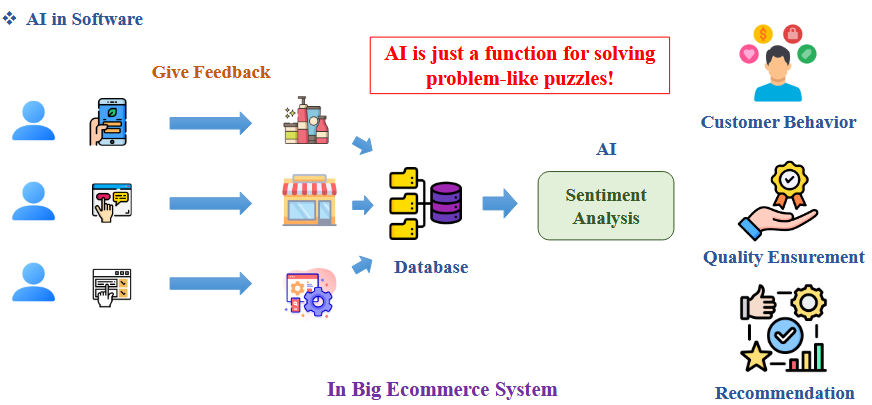
\includegraphics[width=0.8\linewidth]{images/bs_pers.png}
    \caption{Vai trò của AI trong một hệ thống Thương mại điện tử}
\end{figure}

Toàn bộ quy trình ML bắt đầu từ \textbf{Yêu cầu Nghiệp vụ (Business Require)} và đi qua một vòng đời (life cycle) hoàn chỉnh. Để đảm bảo chất lượng (Quality Ensurement) và giám sát (Monitoring) mô hình AI một cách hiệu quả, doanh nghiệp phải có khả năng trả lời các câu hỏi:
\begin{itemize}
    \item Mô hình đang chạy trên production được huấn luyện từ dữ liệu nào?
    \item Khi mô hình dự đoán sai, làm thế nào để tái lập (reproduce) lỗi đó?
    \item Nếu dữ liệu mới làm giảm hiệu suất, làm sao để quay lại phiên bản mô hình ổn định trước đó?
\end{itemize}
Data versioning cung cấp khả năng \textbf{truy xuất nguồn gốc (lineage)} này, cho phép theo dõi chính xác code nào, dữ liệu nào, tham số nào đã tạo ra mô hình nào.

\begin{figure}[H]
    \centering
    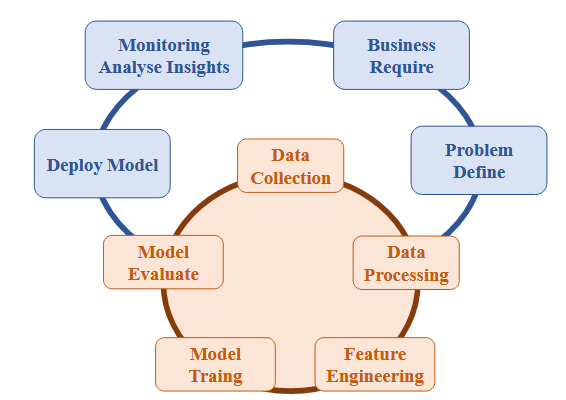
\includegraphics[width=0.7\linewidth]{images/cv_lifecycle.png}
    \caption{Vòng đời Machine Learning (ML Life Cycle)}
\end{figure}

\subsubsection{Góc nhìn MLOps}
MLOps tập trung vào việc tự động hóa và tinh gọn quy trình (pipeline) để chuyển giao mô hình từ môi trường nghiên cứu (Research Environment) sang môi trường triển khai (AI Service). Quy trình này bao gồm các bước lặp đi lặp lại như Xử lý dữ liệu (Data Handling), Huấn luyện mô hình (Model Training), và Đánh giá mô hình (Model Evaluation).

\begin{figure}[H]
    \centering
    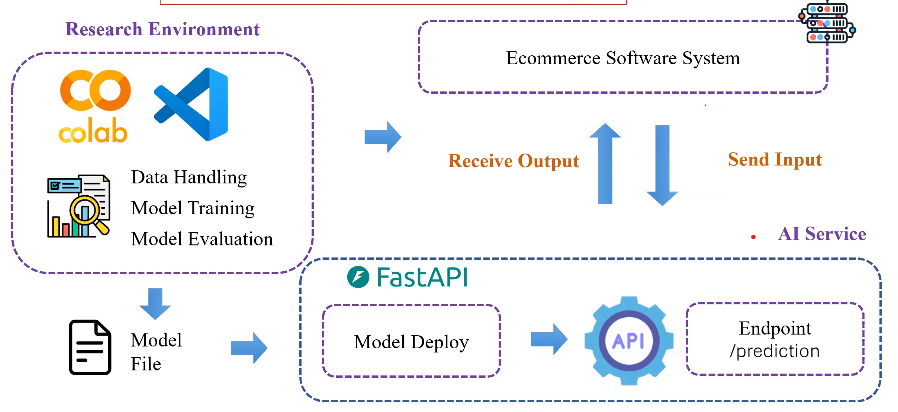
\includegraphics[width=0.9\linewidth]{images/mlop_pipeline.png}
    \caption{Quy trình MLOps cơ bản}
\end{figure}

Data versioning là thành phần quan trọng trả lời câu hỏi "Ở đâu và tại sao chúng ta cần phiên bản hóa dữ liệu?". Nó giúp tự động hóa việc quản lý các "đầu ra" (artifacts) của mỗi bước (như dữ liệu đã xử lý, tệp mô hình, tệp chỉ số) và đảm bảo tính nhất quán giữa các môi trường, đặc biệt là khi làm việc nhóm.


\subsection{Ví dụ thực tế: Thử nghiệm mô hình Time Series}

\subsubsection{Khi KHÔNG có Data Versioning (Cách làm thủ công)}
Hãy tưởng tượng nhóm của bạn đang phát triển một mô hình dự báo chuỗi thời gian (time-series) phức tạp. Quy trình này tạo ra vô số tệp: `dataset files` (dữ liệu gốc), `parameters files` (tham số), `checkpoint files` (điểm kiểm tra mô hình), và `dataset augment files` (dữ liệu tăng cường).

\begin{figure}[H]
    \centering
    \begin{subfigure}{0.48\textwidth}
        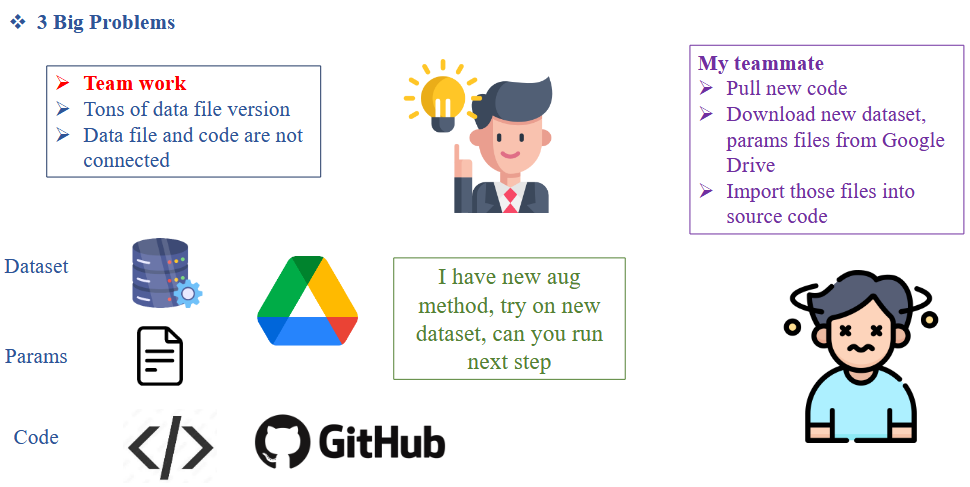
\includegraphics[width=\linewidth]{images/3problems.png}
        \caption{Vấn đề khi làm việc nhóm thủ công}
    \end{subfigure}
    \hfill
    \begin{subfigure}{0.48\textwidth}
        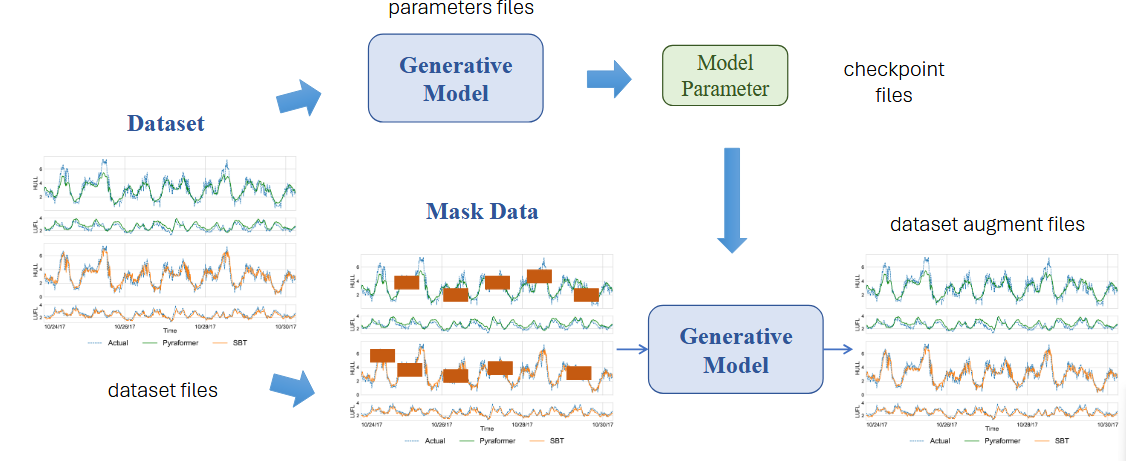
\includegraphics[width=\linewidth]{images/timeseries.png}
        \caption{Pipeline sinh ra nhiều phiên bản tệp}
    \end{subfigure}
    \caption{Sự hỗn loạn khi quản lý thủ công các tệp dữ liệu và thử nghiệm}
\end{figure}

Khi một thành viên trong nhóm ("My teammate") muốn chạy thử nghiệm mới, quy trình của họ rất vất vả:
\begin{enumerate}
    \item \textbf{Pull new code}: Tải code mới nhất từ GitHub.
    \item \textbf{Download new dataset/params}: Truy cập Google Drive, tìm đúng tệp dữ liệu, tệp tham số mới nhất và tải về thủ công.
    \item \textbf{Import files}: Sao chép các tệp này vào đúng thư mục trong source code.
\end{enumerate}
Điều này dẫn đến 3 vấn đề lớn: (1) Có quá nhiều phiên bản tệp dữ liệu, (2) Code và dữ liệu không được kết nối với nhau, và (3) Gây cản trở khi làm việc nhóm. Mọi người sẽ bối rối tự hỏi "Tệp \texttt{cnn\_ettm1\_mix1\_mask025.pkl} này được huấn luyện từ dữ liệu nào?".

\subsubsection{Khi CÓ Data Versioning (với DVC)}
Khi sử dụng một công cụ như DVC, quy trình trên được đơn giản hóa triệt để.
\begin{enumerate}
    \item \textbf{git pull}: Thành viên nhóm tải code mới. Lần này, code mới bao gồm các tệp \texttt{.dvc} (siêu dữ liệu) nhỏ nhẹ trỏ đến dữ liệu.
    \item \textbf{dvc pull}: Họ chỉ cần chạy lệnh này. DVC sẽ đọc các tệp \texttt{.dvc}, tự động tìm và tải về đúng phiên bản dữ liệu, tham số, và mô hình tương ứng với phiên bản code đó từ bộ lưu trữ (ví dụ: S3, Google Drive, hoặc SSH).
\end{enumerate}
Bằng cách này, DVC giải quyết vấn đề "disconnected" bằng cách liên kết code và dữ liệu một cách chặt chẽ thông qua các \texttt{commit}. Mọi thử nghiệm đều được ghi lại, nhất quán và có thể \textbf{tái lập (reproducible)} một cách chính xác bất cứ lúc nào.

% --- PHẦN 2 ---
\section{Phần 2: Thách thức trong Quản lý Dữ liệu và Code}
Các nhóm gặp phải các vấn đề khi xử lý nhiều phiên bản thử nghiệm (experiment versions) và các tập dữ liệu (datasets) lớn. Các vấn đề bao gồm tệp dữ liệu và code không được kết nối với nhau, nhiều bộ dữ liệu, tham số (parameters) và các điểm kiểm tra mô hình (model checkpoints). Khó khăn trong việc theo dõi tệp dữ liệu hoặc tham số nào tương ứng với các phiên bản mô hình cụ thể. Cần có một hệ thống quản lý phiên bản (version control) một cách có hệ thống để quản lý các bộ dữ liệu, tệp cấu hình (configurations), mô hình và kết quả đánh giá một cách gắn kết.

% --- PHẦN 3 ---
\section{Phần 3: Giới thiệu về Data Version Control (DVC)}
DVC (Data Version Control) là một công cụ mã nguồn mở được thiết kế để quản lý dữ liệu và các dự án Machine Learning, hoạt động song song để bổ trợ cho Git.
% \cite{dvc_org_website}. % Bỏ comment dòng này nếu bạn có tệp .bib

\subsection{Workflow Quản lý Phiên bản Dữ liệu}
Một workflow phiên bản hóa dữ liệu (Data Versioning) là một vòng lặp quản lý liên tục. Quy trình này bắt đầu từ \textbf{Model Training} (Huấn luyện Mô hình), sử dụng một bộ \texttt{Data Config} (cấu hình dữ liệu) và \texttt{Model (params)} (tham số mô hình) cụ thể. Toàn bộ tài sản này (dữ liệu, tham số, kết quả đánh giá) được hệ thống \textbf{Data \& Model Management} theo dõi và lưu trữ.

Khi có dữ liệu mới (\texttt{New Data}) hoặc thay đổi cấu hình (\texttt{Diff Config}), quy trình \textbf{Continuos Training} (Huấn luyện Liên tục) sẽ được kích hoạt để tạo ra mô hình mới (\texttt{New Model}) và kết quả đánh giá mới (\texttt{New Eval result}). Phiên bản mới này lại tiếp tục được hệ thống quản lý, hoặc sẵn sàng cho việc \textbf{Model Deployment} (Triển khai).

\begin{figure}[H]
    \centering
    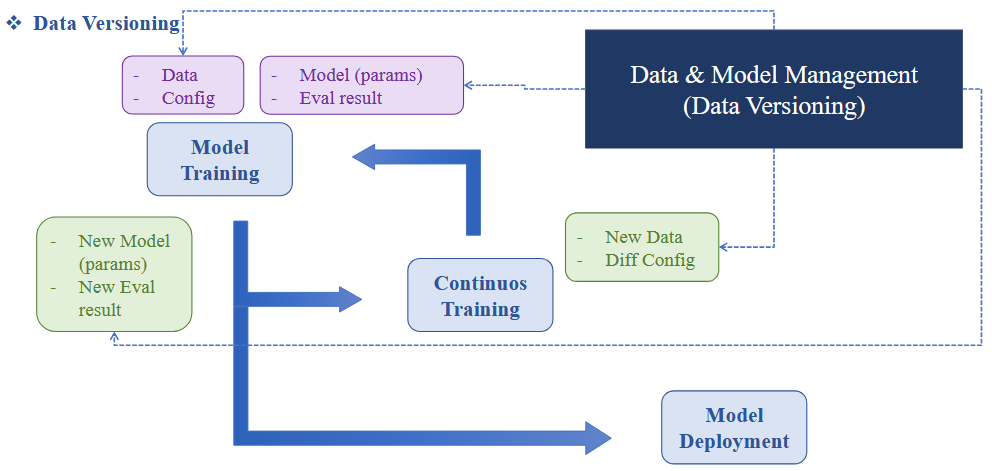
\includegraphics[width=0.8\linewidth]{images/dv_managements.png}
    \caption{Workflow quản lý dữ liệu và mô hình trong MLOps}
\end{figure}

\subsection{So sánh DVC và Giới thiệu chi tiết}
Trên thị trường có nhiều công cụ để phiên bản hóa dữ liệu như Delta Lake, Pachyderm, và DVC. Tuy nhiên, DVC trở nên rất phổ biến vì các lý do chính:
\begin{itemize}
    \item \textbf{Mã nguồn mở}: Sử dụng giấy phép Apache 2.0.
    \item \textbf{Độc lập với định dạng}: \textbf{Data Format Agnostic}, nghĩa là nó có thể quản lý bất kỳ loại tệp nào (model, .csv, .parquet, hình ảnh...).
    \item \textbf{Độc lập với lưu trữ}: \textbf{Cloud/Storage Agnostic}, hỗ trợ hầu hết các nền tảng lưu trữ phổ biến như S3, GCP, Azure, SSH.
    \item \textbf{Dễ sử dụng}: \textbf{Simple to Use}, vì có các lệnh tương tự Git.
\end{itemize}

\begin{figure}[H]
    \centering
    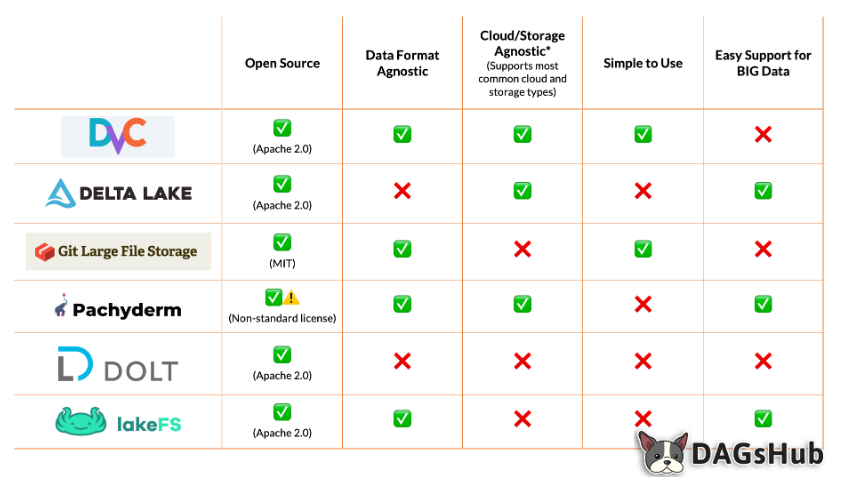
\includegraphics[width=1.0\linewidth]{images/dv_soft.png}
    \caption{So sánh các công cụ Data Version Control phổ biến}
\end{figure}

Về cơ bản, DVC là một nền tảng khoa học dữ liệu cho phép bạn liên kết \texttt{code}, \texttt{data} (dữ liệu), và \texttt{configuration} (cấu hình) để tạo ra các \texttt{model} (mô hình) có thể tái lập (reproducible).

\begin{figure}[H]
    \centering
    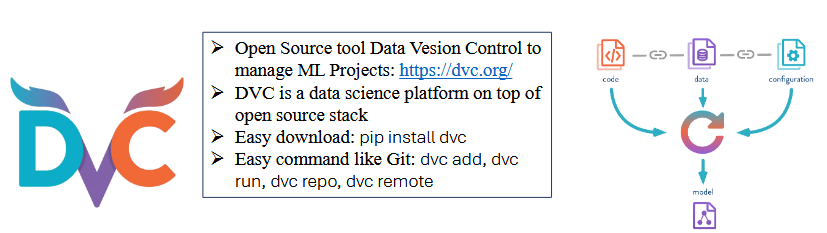
\includegraphics[width=1.0\linewidth]{images/what_dvc.png}
    \caption{DVC liên kết Code, Data, và Configuration để quản lý Model}
\end{figure}

\subsubsection{DVC khác Git như thế nào?}
Điểm khác biệt cốt lõi là: \textbf{Git quản lý Code} (mã nguồn), trong khi \textbf{DVC quản lý Data} (dữ liệu).

Git không được thiết kế để xử lý các tệp lớn (ví dụ: mô hình 500MB). Khi bạn dùng DVC, quy trình làm việc (Local/Remote) sẽ được tách biệt rõ ràng:
\begin{itemize}
    \item \textbf{Git (Code)}: Bạn dùng \texttt{git push/pull} để đồng bộ code (ví dụ: \texttt{train.py}) và các tệp \texttt{.dvc} siêu dữ liệu (chỉ nặng vài KB) lên máy chủ Git (như GitHub, GitLab).
    \item \textbf{DVC (Data)}: Bạn dùng \texttt{dvc push/pull} để đồng bộ các tệp dữ liệu lớn thực tế (ví dụ: \texttt{model.pkl} 500MB) lên một máy chủ lưu trữ (Storage) riêng biệt (như S3, Azure, Google Cloud, SSH).
\end{itemize}

Tệp \texttt{model.pkl.dvc} (1KB) mà Git theo dõi chỉ là một "con trỏ" (pointer) trỏ đến tệp \texttt{model.pkl} (500MB) thực sự được DVC quản lý. Điều này giữ cho kho Git của bạn luôn nhỏ gọn và nhanh chóng.

\begin{figure}[H]
    \centering
    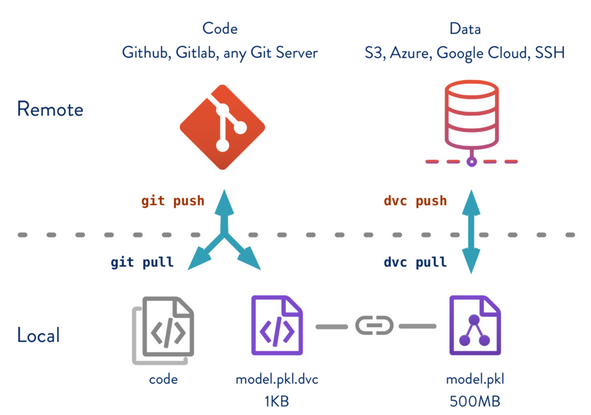
\includegraphics[width=0.7\linewidth]{images/git_v_dvc.png}
    \caption{DVC và Git hoạt động song song: Git quản lý Code, DVC quản lý Data}
\end{figure}

Sự tương đồng về câu lệnh (ví dụ: \texttt{dvc add}, \texttt{dvc push}, \texttt{dvc pull}) khiến DVC rất dễ tiếp cận cho bất kỳ ai đã quen thuộc với Git.

\begin{figure}[H]
    \centering
    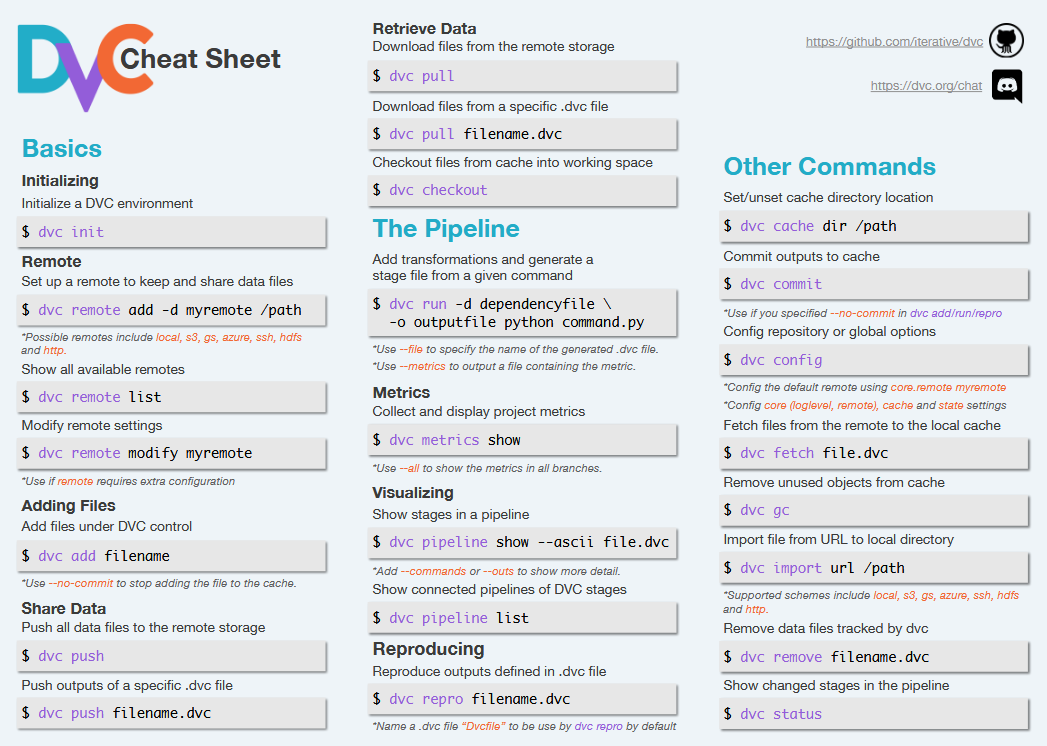
\includegraphics[width=1.0\linewidth]{images/dvc_commands.png}
    \caption{DVC Cheat Sheet cho thấy sự tương đồng với các lệnh Git}
\end{figure}

\subsection{Quy trình DVC Pipeline hoàn chỉnh}
Một DVC pipeline hoàn chỉnh cho phép bạn tự động hóa toàn bộ quy trình ML và đảm bảo tính tái lập (reproducibility). Trung tâm của pipeline này là tệp \texttt{dvc.yaml}.

\subsubsection{1. Định nghĩa Pipeline (dvc.yaml)}
Tệp \texttt{dvc.yaml} là nơi bạn định nghĩa tất cả các \textbf{stages} (giai đoạn) của quy trình ML. Mỗi stage giống như một bước trong "công thức" của bạn. Một stage thường bao gồm:
\begin{itemize}
    \item \texttt{cmd}: Lệnh thực thi (ví dụ: \texttt{python train.py}).
    \item \texttt{deps}: Các tệp phụ thuộc (dependencies) là đầu vào của stage, ví dụ như code (`train.py`) hoặc dữ liệu thô (`data/raw.csv`).
    \item \texttt{params}: Các tham số (parameters), thường được định nghĩa trong tệp \texttt{params.yaml} (ví dụ: learning rate, số epochs).
    \item \texttt{outs}: Các tệp đầu ra (outputs) mà stage này tạo ra, ví dụ như mô hình đã huấn luyện (\texttt{model.pkl}) hoặc dữ liệu đã xử lý.
\end{itemize}

\subsubsection{2. Thực thi Pipeline (dvc repro)}
Khi bạn chạy lệnh \texttt{dvc repro}, DVC sẽ thực hiện một việc rất thông minh:
Nó kiểm tra tệp \texttt{dvc.yaml} và so sánh \textbf{hash} (một chuỗi định danh duy nhất) của các tệp \texttt{deps} và \texttt{params} hiện tại với thông tin được lưu trong tệp \texttt{dvc.lock}.

\begin{itemize}
    \item Tệp \texttt{dvc.lock} lưu lại "dấu vân tay" (hash) của các tệp \texttt{deps}, \texttt{params}, và \texttt{outs} từ lần chạy thành công trước đó.
    \item Nếu hash của bất kỳ tệp \texttt{deps} (ví dụ: bạn sửa code \texttt{train.py}) hoặc bất kỳ \texttt{params} nào thay đổi, DVC sẽ nhận ra stage đó là "lỗi thời" (outdated) và \textbf{chỉ chạy lại stage đó} cùng các stage phụ thuộc vào nó.
    \item Nếu không có gì thay đổi, DVC sẽ không chạy gì cả, giúp tiết kiệm thời gian tính toán.
\end{itemize}
Đây chính là cách DVC đảm bảo rằng mô hình của bạn luôn nhất quán với code và dữ liệu đã tạo ra nó.

\subsection{Các khái niệm DVC cốt lõi cần nhớ}
Đây là những ghi chú quan trọng và các khái niệm cần nhắc lại (từ các câu hỏi quiz) trước khi đi vào thực hành.

\subsubsection{Quy trình làm việc chuẩn: DVC trước, Git sau}
Đây là quy tắc quan trọng nhất. Khi bạn có một tệp dữ liệu lớn (ví dụ: \texttt{data.zip}):
\begin{enumerate}
    \item \textbf{`dvc add data.zip`}: Lệnh này bảo DVC bắt đầu theo dõi \texttt{data.zip}. DVC sao chép tệp này vào kho lưu trữ cục bộ (\texttt{.dvc/cache}) và tạo ra một tệp siêu dữ liệu (pointer) nhỏ tên là \texttt{data.zip.dvc}.
    \item \textbf{`git add data.zip.dvc`}: Bạn dùng Git để theo dõi tệp pointer \texttt{.dvc} (chỉ vài KB), \textbf{KHÔNG BAO GIỜ} `git add` tệp \texttt{data.zip} gốc.
    \item \textbf{`git commit -m "Track new data"`}: Lưu lại trạng thái của tệp pointer.
\end{enumerate}
Nếu bạn `git add` tệp lớn trước, kho Git của bạn sẽ bị phình to và DVC sẽ không thể quản lý tệp đó.

\subsubsection{git push vs. dvc push}
Đây là điểm khác biệt cốt lõi (như trong hình \texttt{git\_v\_dvc.png}):
\begin{itemize}
    \item \textbf{`git push`}: Chỉ đẩy code (`.py`) và các tệp siêu dữ liệu/con trỏ (`.dvc`, `dvc.yaml`) lên máy chủ Git (như GitHub).
    \item \textbf{`dvc push`}: Đẩy các tệp dữ liệu lớn thực tế (mà DVC đang theo dõi) từ cache cục bộ (\texttt{.dvc/cache}) lên kho lưu trữ từ xa (Remote Storage) như AWS S3, GCS, hoặc SSH.
\end{itemize}

\begin{figure}[H]
    \centering
    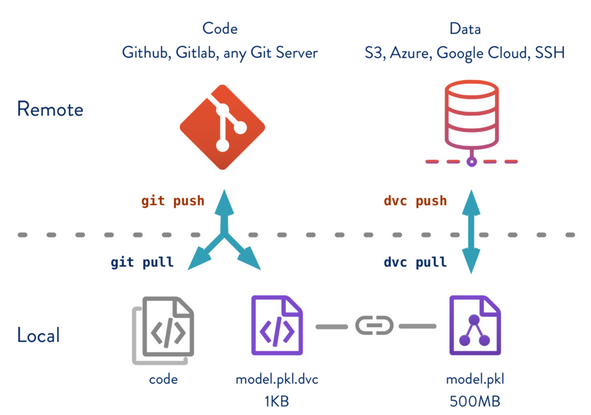
\includegraphics[width=0.7\linewidth]{images/git_v_dvc.png}
    \caption{Git quản lý Code/Metadata, DVC quản lý Data thực tế}
\end{figure}

\subsubsection{dvc pull vs. dvc checkout}
Khi làm việc nhóm, bạn sẽ dùng hai lệnh này:
\begin{itemize}
    \item \textbf{`dvc pull`}: Tải dữ liệu từ Remote Storage (ví dụ: S3) về kho lưu trữ cục bộ (Local Cache) của bạn (thư mục \texttt{.dvc/cache}).
    \item \textbf{`dvc checkout`}: Đồng bộ hóa dữ liệu từ Local Cache ra thư mục làm việc (workspace) của bạn. Lệnh này đọc các tệp \texttt{.dvc} trong workspace và tạo liên kết (symlink) đến các tệp tương ứng trong cache. Bạn thường chạy lệnh này sau khi \texttt{git checkout} một branch mới.
\end{itemize}

\subsubsection{Điều kiện tiên quyết cho DVC Pipeline}
Trước khi có thể chạy \texttt{dvc repro}, bạn cần đảm bảo:
\begin{enumerate}
    \item Dự án đã được khởi tạo là một kho Git (\texttt{git init}).
    \item Đã cài đặt các thư viện cần thiết (ví dụ: \texttt{pip install dvc dvc-s3}).
    \item Đã định nghĩa các stage trong tệp \texttt{dvc.yaml}.
    \item (Tùy chọn) Đã kết nối với kho lưu trữ từ xa bằng lệnh \texttt{dvc remote add}, ví dụ: \\ \texttt{dvc remote add -d my-s3-storage s3://my-bucket/dvc-storage}.
\end{enumerate}

% --- PHẦN 4 ---
\section{Phần 4: Case Study: Triển khai DVC cho Dataset MNIST}
Chúng ta sẽ thực hiện một case study từng bước để thấy DVC và Git hoạt động song song như thế nào để quản lý các phiên bản thử nghiệm (dữ liệu và mô hình).

\subsection{Bước 1: Thiết lập Dự án và Git}
Đầu tiên, chúng ta tạo thư mục dự án, cấu trúc thư mục con, môi trường \texttt{conda}, và quan trọng nhất là khởi tạo kho Git.

\begin{lstlisting}[language=bash]
# 1. Tạo thư mục dự án và cấu trúc cơ bản
$ mkdir dvc-mnist-demo
$ cd dvc-mnist-demo
$ mkdir data/raw models scripts

# 2. Tạo môi trường conda và cài đặt thư viện
$ conda create -n dvc_mnist python=3.11
$ conda activate dvc_mnist
$ pip install -r requirements.txt

# 3. Khởi tạo Git và commit lần đầu
$ git init
$ git add .
$ git commit -m "Init project"
\end{lstlisting}

\begin{figure}[H]
    \centering
    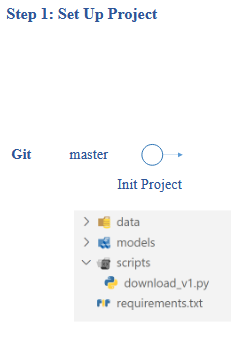
\includegraphics[width=1.0\linewidth]{images/p3.png}
    \caption{Trạng thái Git và cấu trúc file ban đầu}
\end{figure}

\subsection{Bước 2: Tải Dataset V1 và Theo dõi bằng DVC}
Tiếp theo, chúng ta tải phiên bản đầu tiên của dataset (Full MNIST) và dùng DVC để bắt đầu theo dõi nó.

\begin{lstlisting}[language=bash]
# 1. Tải dữ liệu (60000 mẫu)
$ python scripts/download_v1.py

# 2. Khởi tạo DVC trong dự án
$ dvc init

# 3. Yêu cầu DVC theo dõi các tệp dữ liệu lớn
$ dvc add data/raw/x_train_v1.npy data/raw/y_train_v1.npy data/raw/x_test.npy data/raw/y_test.npy
\end{lstlisting}
Lệnh \texttt{dvc add} sẽ tạo ra các tệp \texttt{.dvc} (con trỏ) siêu dữ liệu và tự động thêm các tệp \texttt{.npy} lớn vào \texttt{.gitignore}.

\subsection{Bước 3: Commit Phiên bản Dữ liệu V1}
Giờ chúng ta commit các tệp \texttt{.dvc} (con trỏ) vào Git để lưu lại "phiên bản" dữ liệu này.

\begin{lstlisting}[language=bash]
# Add các tệp .dvc (con trỏ) và tệp .gitignore đã được DVC cập nhật
$ git add data/raw/.gitignore data/raw/x_train_v1.npy.dvc data/raw/y_train_v1.npy.dvc data/raw/x_test.npy.dvc data/raw/y_test.npy.dvc

# Commit để chốt phiên bản V1
$ git commit -m "Version 1: Full MNIST dataset"
\end{lstlisting}

\begin{figure}[H]
    \centering
    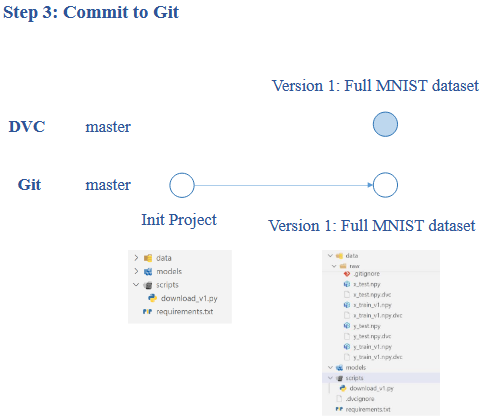
\includegraphics[width=1.0\linewidth]{images/p7.png}
    \caption{Lịch sử Git và DVC song song sau khi commit dữ liệu V1}
\end{figure}

\subsection{Bước 4: Huấn luyện và Theo dõi Mô hình V1}
Với dữ liệu V1, chúng ta huấn luyện mô hình đầu tiên và lại dùng DVC để theo dõi các tệp mô hình và chỉ số (metrics) đầu ra.

\begin{lstlisting}[language=bash]
# 1. (Tùy chọn) Tạo symbolic link để script train.py đọc dữ liệu
$ cd data/raw
$ mklink x_train.npy x_train_v1.npy
$ mklink y_train.npy y_train_v1.npy
$ cd ../..

# 2. Chạy huấn luyện (trên 60000 mẫu, đạt 0.9319 accuracy)
$ python scripts/train.py

# 3. Yêu cầu DVC theo dõi các tệp đầu ra (mô hình và chỉ số)
$ dvc add models/model.npy
$ dvc add models/metrics.json

# 4. Commit các con trỏ .dvc của mô hình V1 vào Git
$ git add .
$ git commit -m "Model v1: Full dataset accuracy"
\end{lstlisting}

\begin{figure}[H]
    \centering
    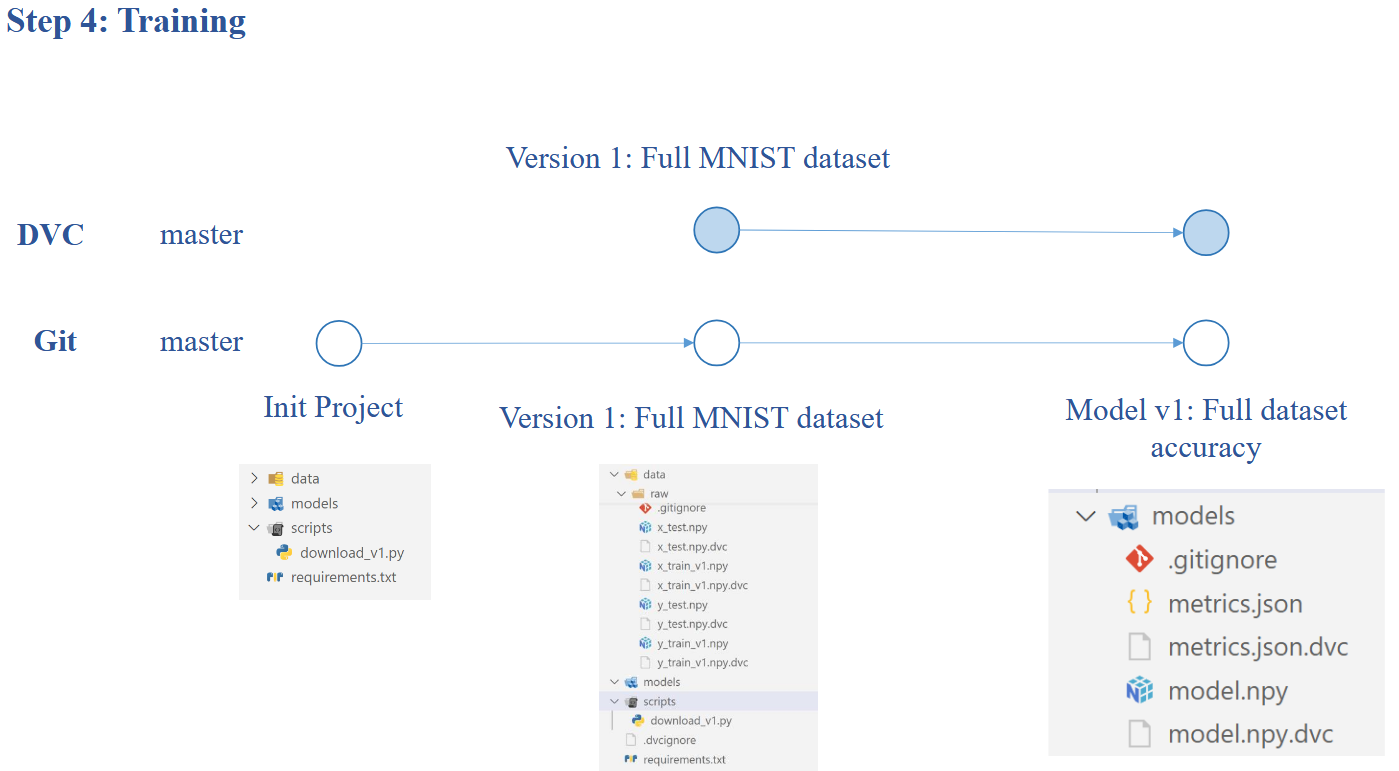
\includegraphics[width=1.0\linewidth]{images/p10.png}
    \caption{Toàn bộ lịch sử Git và DVC sau khi huấn luyện và commit Mô hình V1}
\end{figure}


\subsection{Bước 5: Tạo Phiên bản Dữ liệu V2}
Bây giờ, chúng ta giả lập một thử nghiệm mới bằng cách tạo phiên bản dữ liệu thứ hai (chỉ 1000 mẫu).

\begin{lstlisting}[language=bash]
# 1. Chạy script download_v2.py để tạo dữ liệu V2
$ python scripts/download_v2.py

# 2. Yêu cầu DVC theo dõi các tệp dữ liệu V2 mới
$ dvc add data/raw/x_train_v2.npy
$ dvc add data/raw/y_train_v2.npy

# 3. Commit các con trỏ .dvc của V2 vào Git
$ git add .
$ git commit -m "Dataset V2"
\end{lstlisting}

\begin{figure}[H]
    \centering
    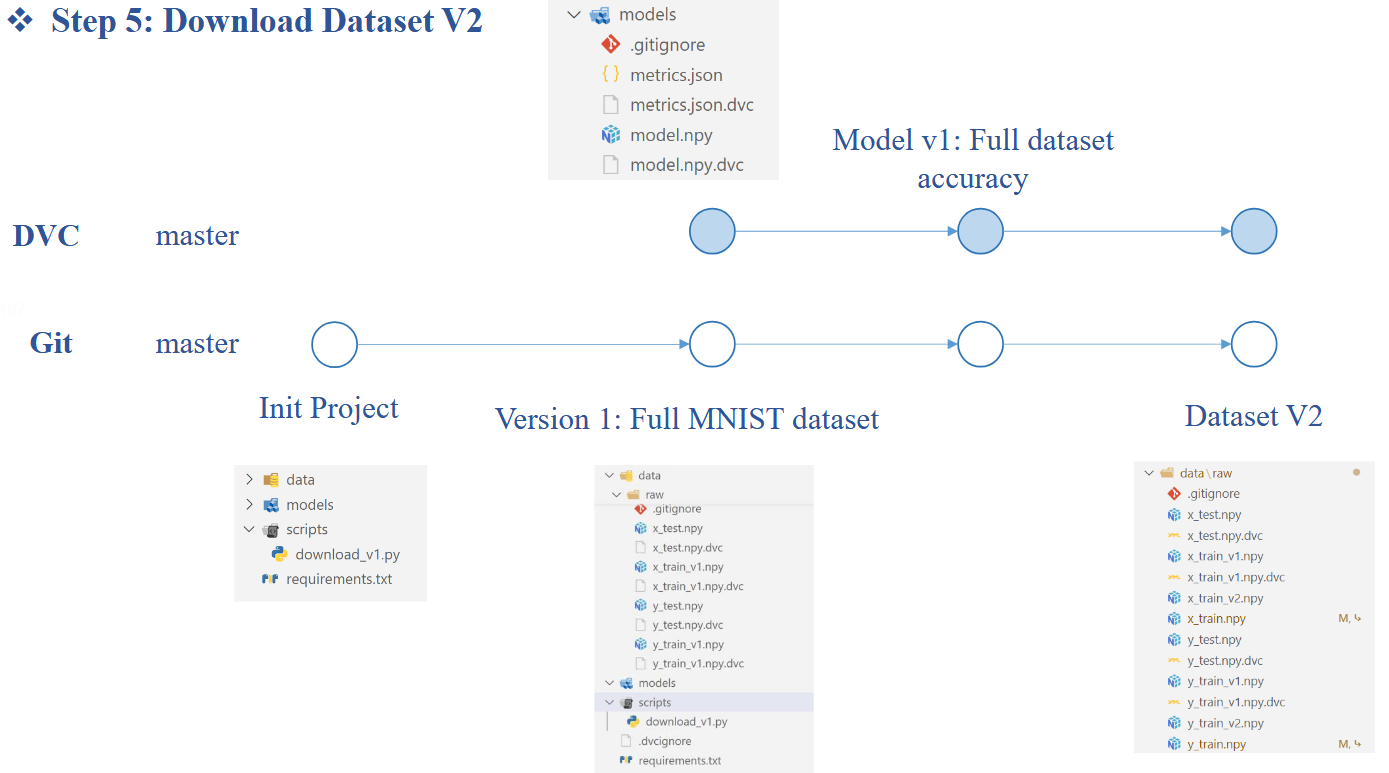
\includegraphics[width=1.0\linewidth]{images/p14.png}
    \caption{Lịch sử Git và DVC sau khi thêm "Dataset V2"}
\end{figure}

\subsection{Bước 6: Huấn luyện Mô hình V2}
Chúng ta lặp lại quy trình huấn luyện, nhưng lần này sử dụng dữ liệu V2 (bằng cách thay đổi symbolic link) để tạo ra mô hình V2.

\begin{lstlisting}[language=bash]
# 1. Cập nhật symbolic link để trỏ tới dữ liệu V2
$ cd data/raw
$ del x_train.npy y_train.npy
$ mklink x_train.npy x_train_v2.npy
$ mklink y_train.npy y_train_v2.npy
$ cd ../..

# 2. Chạy huấn luyện (trên 1000 mẫu, đạt 0.8047 accuracy)
$ python scripts/train.py
\end{lstlisting}

\subsection{Bước 7: Theo dõi Mô hình V2}
Giờ chúng ta theo dõi các tệp mô hình và chỉ số V2 mới.

\begin{lstlisting}[language=bash]
# 1. Yêu cầu DVC theo dõi các tệp mô hình và chỉ số V2
$ dvc add models/model.npy
$ dvc add models/metrics.json

# 2. Commit các con trỏ .dvc của mô hình V2
$ git add .
$ git commit -m "Model v2: Small dataset accuracy"
\end{lstlisting}

\begin{figure}[H]
    \centering
    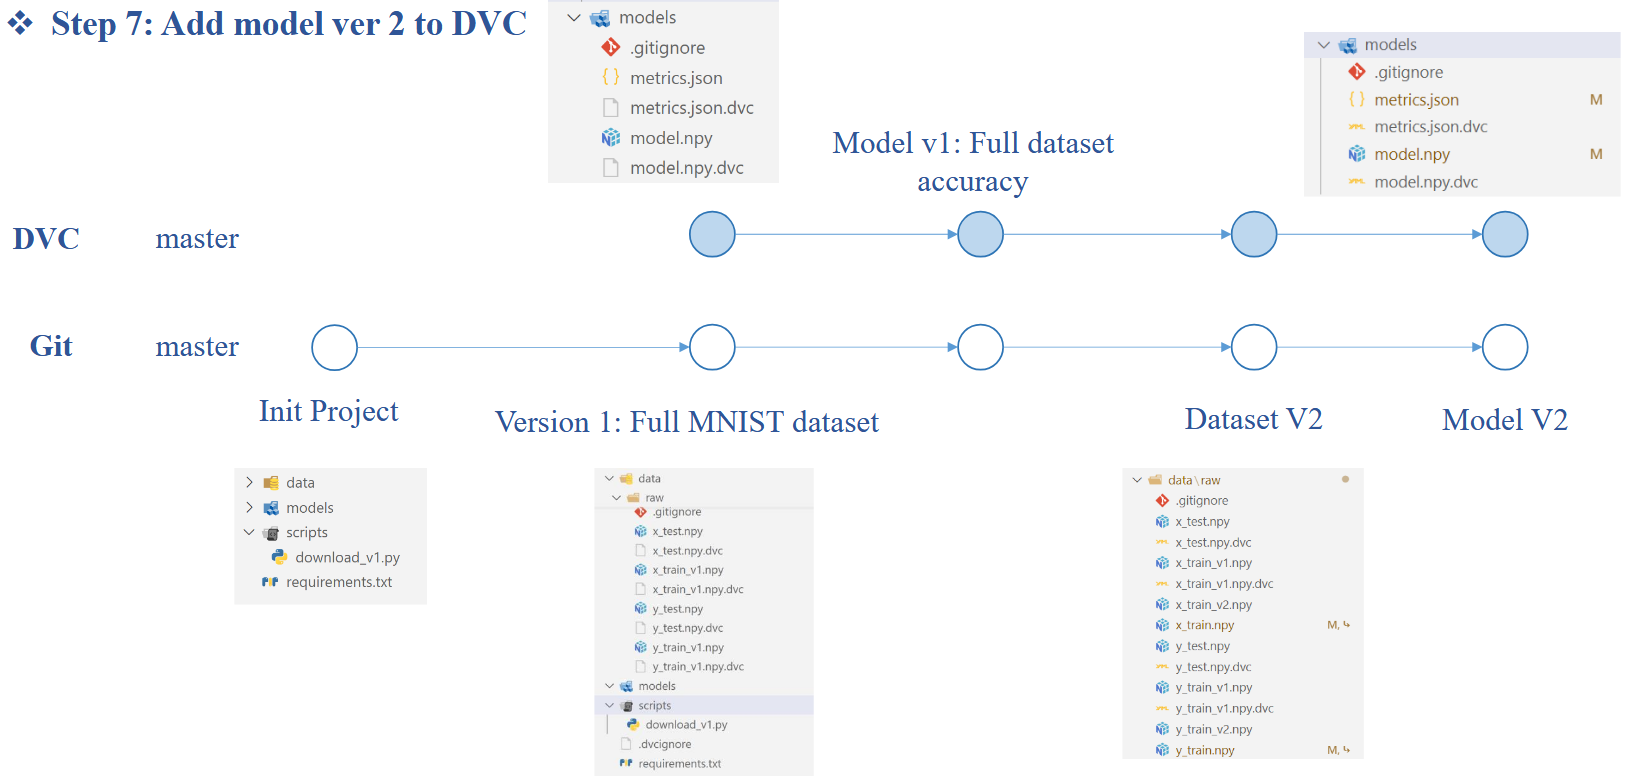
\includegraphics[width=1.0\linewidth]{images/p18.png}
    \caption{Lịch sử Git/DVC hoàn chỉnh với 2 phiên bản dữ liệu và 2 phiên bản mô hình}
\end{figure}

\subsection{Bước 8: Cấu hình Kho lưu trữ (Storage)}
Các tệp dữ liệu lớn thực sự nằm trong cache (\texttt{.dvc/cache}). Để chia sẻ chúng, ta cần thiết lập một kho lưu trữ từ xa (remote storage).

\subsubsection{Sử dụng Local Storage (Lưu trữ Cục bộ)}
Đây là cách đơn giản để chia sẻ cache trong cùng một máy hoặc qua mạng nội bộ.
\begin{lstlisting}[language=bash]
# 1. Tạo một thư mục bên ngoài dự án để làm "storage"
$ mkdir dvc_storage
# 2. Thêm nó làm remote "localremote" (lưu cấu hình vào .dvc/config)
$ dvc remote add -d localremote ./dvc_storage
# 3. Đẩy dữ liệu từ cache (.dvc/cache) lên localremote
$ dvc push
\end{lstlisting}

\subsubsection{Sử dụng Cloud Storage (ví dụ: AWS S3)}
Đây là cách làm phổ biến nhất khi làm việc nhóm.
\begin{lstlisting}[language=bash]
# 1. Cài đặt thư viện hỗ trợ S3
$ pip install dvc-s3
# 2. Thêm S3 bucket làm remote "mys3"
$ dvc remote add -d mys3 s3://dvc-mnist-demo-bucket/data
# 3. Đẩy dữ liệu từ cache lên S3 (remote mặc định)
$ dvc push
\end{lstlisting}

\subsection{Bước 9: Kiểm tra Chuyển đổi Phiên bản}
Đây là sức mạnh lớn nhất của DVC. Chúng ta có thể quay lại bất kỳ thử nghiệm nào trong quá khứ.
Ví dụ, để quay lại commit của Mô hình V1:
\begin{lstlisting}[language=bash]
# 1. Tìm commit_id của V1 (ví dụ: "Model v1: Full dataset accuracy")
$ git log

# 2. Quay lại trạng thái code của commit đó
$ git checkout <commit_id_cua_V1>

# 3. Yêu cầu DVC đồng bộ dữ liệu/mô hình tương ứng với commit đó
$ dvc checkout

# 4. Kiểm tra (sẽ thấy shape của V1 là 60000)
$ python -c "import numpy as np; print('V1 Data shape:', np.load('data/raw/x_train.npy').shape)"
\end{lstlisting}
Nếu bạn \texttt{git checkout master} và \texttt{dvc checkout} một lần nữa, dữ liệu sẽ quay về V2 (1000 mẫu).

\subsection{Bước 10: Push và Clone (Làm việc nhóm)}
Quy trình làm việc nhóm điển hình:
\begin{lstlisting}[language=bash]
# --- Người A (Đẩy dự án lên) ---
# 1. Đẩy code và con trỏ .dvc lên GitHub
$ git remote add origin <your-repository>
$ git push origin master
# 2. Đẩy dữ liệu thực tế lên Cloud Storage
$ dvc push

# --- Người B (Lấy dự án về) ---
# 1. Clone code và con trỏ .dvc từ GitHub
$ git clone <your-repository>
# 2. Kết nối tới Cloud Storage
$ dvc remote add -d mys3 s3://dvc-mnist-demo-bucket/data
# 3. Kéo dữ liệu thực tế từ Cloud Storage về cache
$ dvc pull
\end{lstlisting}

\subsection{Bước 11: Tổng kết Thao tác DVC cơ bản}
Workflow trên minh họa các lệnh DVC cơ bản bạn sẽ sử dụng hàng ngày:

\begin{figure}[H]
    \centering
    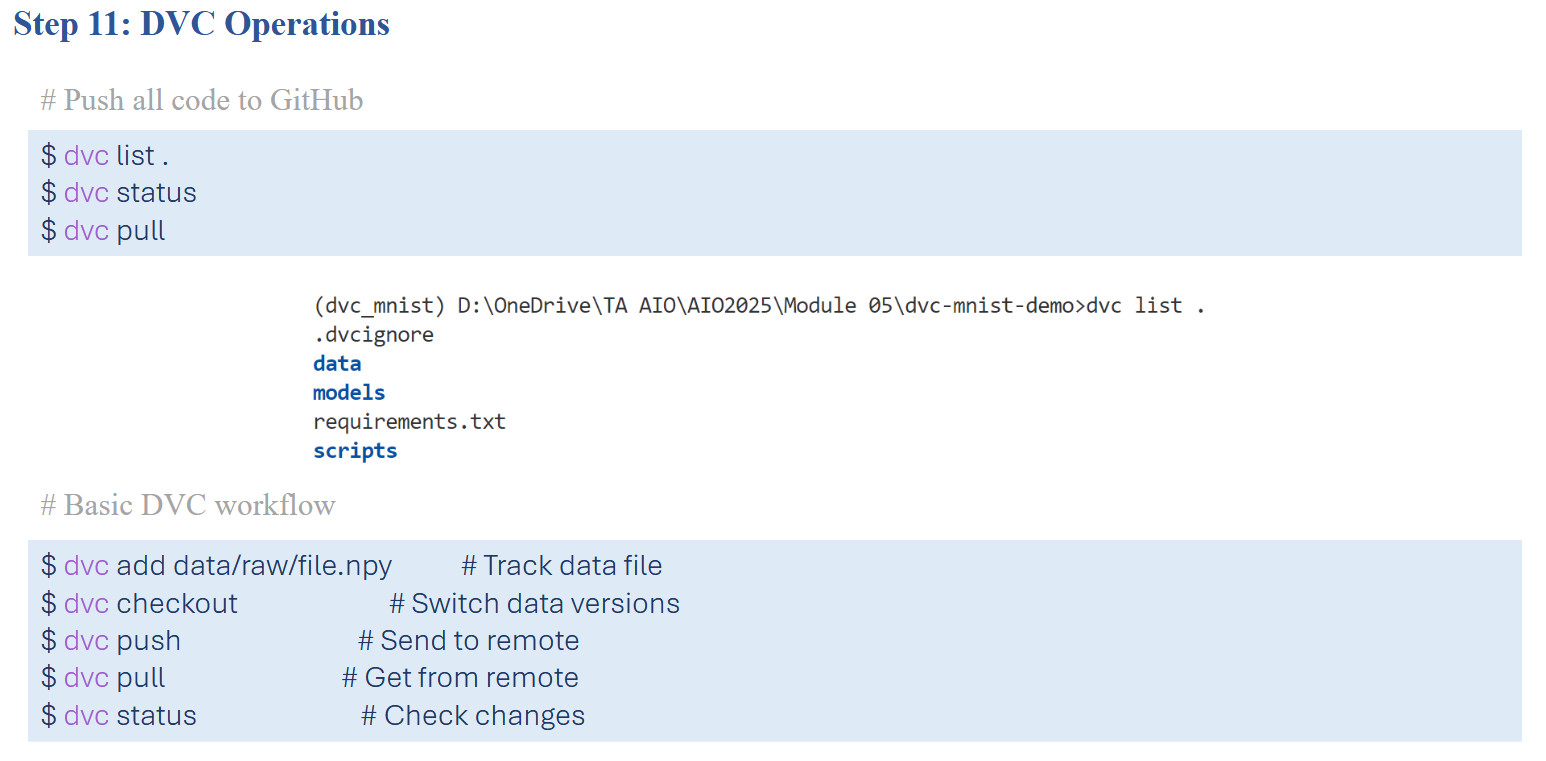
\includegraphics[width=1.0\linewidth]{images/p22.png}
    \caption{Các lệnh DVC workflow cơ bản}
\end{figure}

\begin{lstlisting}[language=bash, commentstyle=\color{gray}]
# Yêu cầu DVC theo dõi một tệp
$ dvc add data/raw/file.npy    # Ghi chú: Track data file

# Đồng bộ dữ liệu từ cache ra thư mục làm việc (khi checkout Git)
$ dvc checkout                 # Ghi chú: Switch data versions

# Đẩy dữ liệu (tệp lớn) từ cache lên kho lưu trữ từ xa (S3, GCS...)
$ dvc push                     # Ghi chú: Send to remote

# Kéo dữ liệu (tệp lớn) từ kho lưu trữ từ xa về cache
$ dvc pull                     # Ghi chú: Get from remote

# Kiểm tra trạng thái các tệp dữ liệu so với commit Git
$ dvc status                   # Ghi chú: Check changes

# Liệt kê các tệp đang được DVC theo dõi trong dự án
$ dvc list .
\end{lstlisting}

% --- PHẦN 5 ---
\section{Phần 5: Tự động hóa Pipelines và Các khái niệm Versioning}
Một trong những tính năng mạnh mẽ nhất của DVC là khả năng tự động hóa toàn bộ quy trình Machine Learning (ML pipeline) thông qua các tệp cấu hình (Configure File).

Tệp cấu hình chính là \texttt{dvc.yaml}. Bạn có thể coi nó như một "bản công thức" hay một "bản kế hoạch chi tiết" cho dự án của bạn. Nó là một tệp văn bản đơn giản mà con người có thể đọc được, thường nằm ở thư mục gốc (root) của dự án. Tệp này định nghĩa tất cả các \textbf{stages} (giai đoạn) trong quy trình của bạn, ví dụ: "bước 1: tải dữ liệu", "bước 2: xử lý dữ liệu", "bước 3: huấn luyện mô hình".

Mục đích của nó là giải quyết vấn đề "phải chạy thủ công" (manual work) và đảm bảo \textbf{khả năng tái lập (reproducibility)}. Thay vì phải nhớ chạy 5 tệp Python theo đúng thứ tự, bạn chỉ cần định nghĩa chúng một lần trong \texttt{dvc.yaml}. Sau đó, DVC sẽ tự động biết phải chạy gì, theo thứ tự nào, và quan trọng nhất: chỉ chạy lại những bước bị ảnh hưởng khi code hoặc dữ liệu của bạn thay đổi, giúp tiết kiệm rất nhiều thời gian.

\subsection{5.1: DVC Automation Pipeline (Quy trình Tự động hóa DVC)}
Hãy xem cách tệp \texttt{dvc.yaml} định nghĩa một pipeline.

\begin{figure}[H]
    \centering
    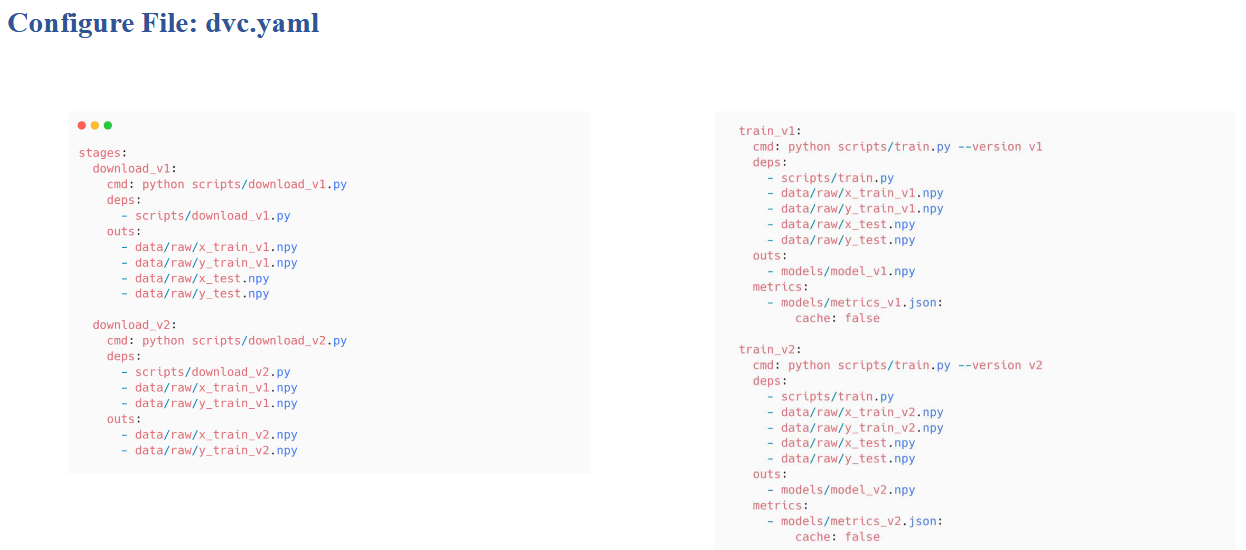
\includegraphics[width=1.0\linewidth]{images/auto1.png}
    \caption{Cấu hình các giai đoạn (stages) trong \texttt{dvc.yaml}}
\end{figure}

Trong tệp \texttt{dvc.yaml}, mọi thứ được tổ chức trong \texttt{stages}:
\begin{itemize}
    \item \textbf{`stages:`}: Khai báo bắt đầu danh sách các giai đoạn.
    \item \textbf{`download_v1:`}: Đây là \textbf{tên} của một stage.
    \item \textbf{`cmd:`}: Lệnh (command) sẽ được thực thi khi chạy stage này (ví dụ: \texttt{python scripts/download\_v1.py}).
    \item \textbf{`deps:`}: Các tệp phụ thuộc (dependencies). DVC sẽ theo dõi các tệp này. Nếu tệp \texttt{scripts/download\_v1.py} thay đổi, DVC sẽ biết stage này "lỗi thời" và cần chạy lại.
    \item \textbf{`outs:`}: Các tệp đầu ra (outputs). Đây là kết quả của stage (ví dụ: \texttt{data/raw/x\_train\_v1.npy}). DVC sẽ tự động theo dõi (giống như \texttt{dvc add}) các tệp này.
\end{itemize}
Bạn có thể thấy các stage \texttt{train_v1} và \texttt{train_v2} phức tạp hơn, chúng phụ thuộc vào cả script (\texttt{train.py}) và dữ liệu đầu vào (ví dụ: \texttt{data/raw/x\_train\_v1.npy}). Điều này tạo ra một chuỗi liên kết, hay một \textbf{DAG (Directed Acyclic Graph)}, nơi DVC hiểu rằng phải chạy \texttt{download_v1} trước rồi mới được chạy \texttt{train_v1}.

\subsubsection{Sử dụng params.yaml để Tối ưu Pipeline}
Việc sao chép và dán các stage \texttt{train_v1} và \texttt{train_v2} (như trong hình trên) rất dễ gây lỗi. Một cách tốt hơn là sử dụng tệp \texttt{params.yaml} để lưu trữ các tham số (hyperparameters).

\begin{figure}[H]
    \centering
    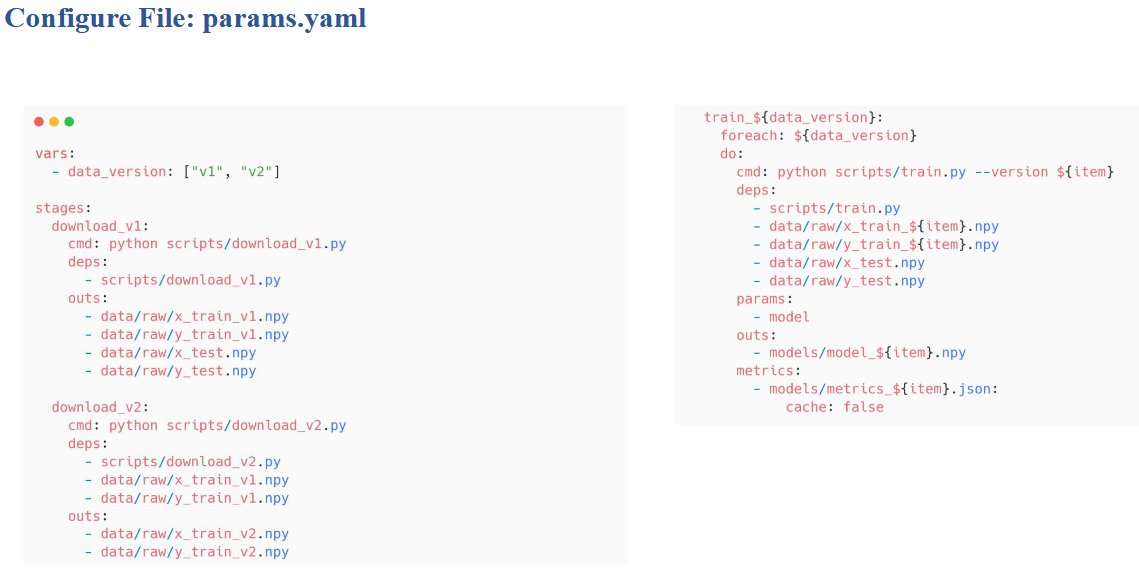
\includegraphics[width=1.0\linewidth]{images/auto3.png}
    \caption{Kết hợp \texttt{dvc.yaml} (phải) và \texttt{params.yaml} (trái)}
\end{figure}

Thay vì định nghĩa hai stage riêng biệt, chúng ta sử dụng "templating" (tạo mẫu):
\begin{enumerate}
    \item \textbf{`params.yaml`}: Chúng ta định nghĩa một biến \texttt{data\_version: ["v1", "v2"]}.
    \item \textbf{`dvc.yaml`}: Chúng ta tạo một stage \texttt{train\_\${data\_version}} (tên stage động).
    \item \textbf{`foreach:`}: DVC sẽ lặp qua từng mục (item) trong \texttt{data\_version}.
    \item \textbf{`\${item}`}: Biến giữ chỗ này sẽ được thay thế bằng "v1" và "v2" khi chạy.
\end{enumerate}
Với cách này, bạn chỉ cần định nghĩa stage \texttt{train} một lần. Nếu sau này bạn muốn thêm "v3", bạn chỉ cần thêm "v3" vào tệp \texttt{params.yaml} mà không cần sửa \texttt{dvc.yaml}.

\subsection{5.2: Ý tưởng của Versioning (Phiên bản hóa)}
Khái niệm cốt lõi của DVC là mở rộng Git workflow (quy trình làm việc của Git) cho dữ liệu và các thử nghiệm (experiments).

\begin{figure}[H]
    \centering
    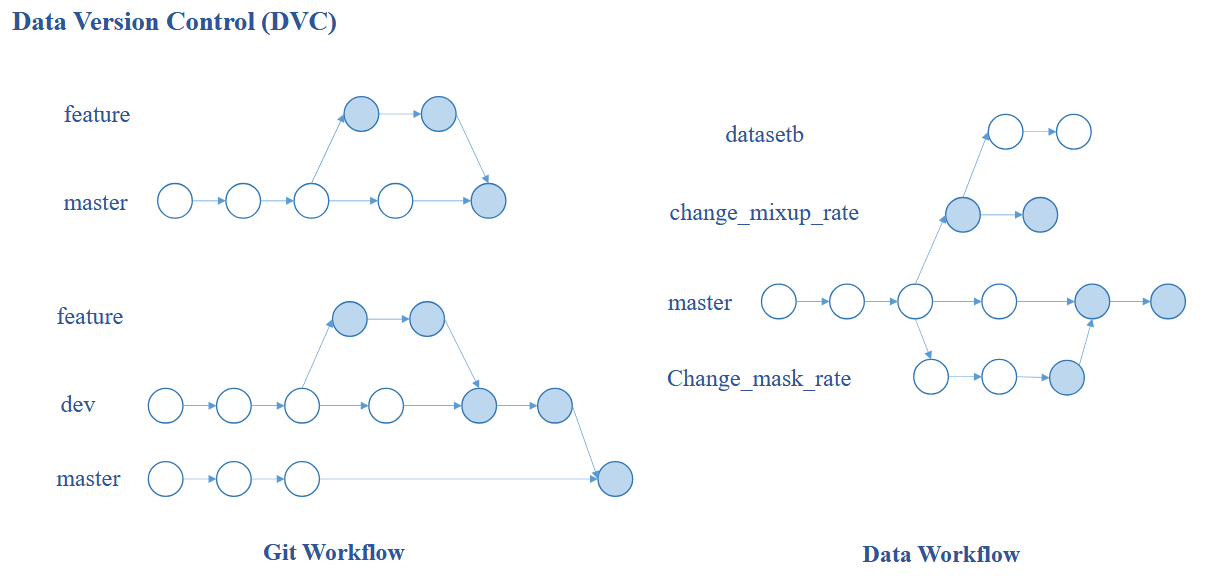
\includegraphics[width=1.0\linewidth]{images/versoning.png}
    \caption{So sánh Git Workflow (trái) và Data Workflow (phải)}
\end{figure}

\begin{itemize}
    \item \textbf{Git Workflow (Bên trái):} Trong phát triển phần mềm, khi muốn phát triển một tính năng mới (feature), bạn tạo một \textbf{nhánh (branch)} mới từ \texttt{master}, thêm code (các commit màu xanh), và khi hoàn thành, bạn gộp (merge) nó trở lại.

    \item \textbf{Data Workflow (Bên phải):} Chúng ta áp dụng ý tưởng tương tự cho các thử nghiệm ML.
    \begin{itemize}
        \item Nhánh \texttt{master} là mô hình chính (production model) của bạn.
        \item Khi bạn muốn thử một ý tưởng mới, ví dụ thay đổi tham số \texttt{mask_rate}, bạn tạo một nhánh Git mới tên là \texttt{Change\_mask\_rate}.
        \item Trên nhánh này, bạn thay đổi tệp \texttt{params.yaml}, sau đó chạy \texttt{dvc repro}. DVC sẽ tạo ra mô hình và chỉ số mới, sau đó bạn \texttt{git commit} các thay đổi đó (ví dụ: \texttt{dvc.lock}).
        \item Tương tự, bạn có thể tạo nhánh \texttt{change\_mixup\_rate} hoặc nhánh \texttt{datasetb} để thử nghiệm dữ liệu mới.
    \end{itemize}
\end{itemize}
Bằng cách này, mỗi nhánh Git đại diện cho một thử nghiệm ML hoàn chỉnh và có thể tái lập. Bạn có thể dễ dàng chuyển đổi giữa các thử nghiệm (\texttt{git checkout}) và so sánh kết quả (\texttt{dvc metrics diff}) mà không làm lộn xộn nhánh \texttt{master} chính.

\printbibliography % Bỏ comment dòng này nếu bạn có tệp .bib

\end{document}